\documentclass{article}
\usepackage{amsfonts,amssymb,amsmath,amsthm}

%% set-style letters
\def\AA{{\mathbb{A}}}
\def\BB{{\mathbb{B}}}
\def\CC{{\mathbb{C}}}
\def\DD{{\mathbb{D}}}
\def\EE{{\mathbb{E}}}
\def\FF{{\mathbb{F}}}
\def\GG{{\mathbb{G}}}
\def\HH{{\mathbb{H}}}
\def\II{{\mathbb{I}}}
\def\JJ{{\mathbb{J}}}
\def\KK{{\mathbb{K}}}
\def\LL{{\mathbb{L}}}
\def\MM{{\mathbb{M}}}
\def\NN{{\mathbb{N}}}
\def\OO{{\mathbb{O}}}
\def\PP{{\mathbb{P}}}
\def\QQ{{\mathbb{Q}}}
\def\RR{{\mathbb{R}}}
\def\SS{{\mathbb{S}}}
\def\TT{{\mathbb{T}}}
\def\UU{{\mathbb{U}}}
\def\VV{{\mathbb{V}}}
\def\WW{{\mathbb{W}}}
\def\XX{{\mathbb{X}}}
\def\YY{{\mathbb{Y}}}
\def\ZZ{{\mathbb{Z}}}

%% calligraphic letters
\def\cA{{\mathcal{A}}}
\def\cB{{\mathcal{B}}}
\def\cC{{\mathcal{C}}}
\def\cD{{\mathcal{D}}}
\def\cE{{\mathcal{E}}}
\def\cF{{\mathcal{F}}}
\def\cG{{\mathcal{G}}}
\def\cH{{\mathcal{H}}}
\def\cI{{\mathcal{I}}}
\def\cJ{{\mathcal{J}}}
\def\cK{{\mathcal{K}}}
\def\cL{{\mathcal{L}}}
\def\cM{{\mathcal{M}}}
\def\cN{{\mathcal{N}}}
\def\cO{{\mathcal{O}}}
\def\cP{{\mathcal{P}}}
\def\cQ{{\mathcal{Q}}}
\def\cR{{\mathcal{R}}}
\def\cS{{\mathcal{S}}}
\def\cT{{\mathcal{T}}}
\def\cU{{\mathcal{U}}}
\def\cV{{\mathcal{V}}}
\def\cW{{\mathcal{W}}}
\def\cX{{\mathcal{X}}}
\def\cY{{\mathcal{Y}}}
\def\cZ{{\mathcal{Z}}}
\def\cKL{{\mathcal{KL}}}

%% bold letters
\def\bA{{\bf{A}}}
\def\bB{{\bf{B}}}
\def\bC{{\bf{C}}}
\def\bD{{\bf{D}}}
\def\bE{{\bf{E}}}
\def\bF{{\bf{F}}}
\def\bG{{\bf{G}}}
\def\bH{{\bf{H}}}
\def\bI{{\bf{I}}}
\def\bJ{{\bf{J}}}
\def\bK{{\bf{K}}}
\def\bL{{\bf{L}}}
\def\bM{{\bf{M}}}
\def\bN{{\bf{N}}}
\def\bO{{\bf{O}}}
\def\bP{{\bf{P}}}
\def\bQ{{\bf{Q}}}
\def\bR{{\bf{R}}}
\def\bS{{\bf{S}}}
\def\bT{{\bf{T}}}
\def\bU{{\bf{U}}}
\def\bV{{\bf{V}}}
\def\bW{{\bf{W}}}
\def\bX{{\bf{X}}}
\def\bY{{\bf{Y}}}
\def\bZ{{\bf{Z}}}
\def\ba{{\bf{a}}}
\def\bb{{\bf{b}}}
\def\bc{{\bf{c}}}
\def\bd{{\bf{d}}}
\def\be{{\bf{e}}}
\def\boldf{{\bf{f}}} %different
\def\bg{{\bf{g}}}
\def\bh{{\bf{h}}}
\def\bi{{\bf{i}}}
\def\bj{{\bf{j}}}
\def\bk{{\bf{k}}}
\def\bl{{\bf{l}}}
\def\bm{{\bf{m}}}
\def\bn{{\bf{n}}}
\def\bo{{\bf{o}}}
\def\bp{{\bf{p}}}
\def\bq{{\bf{q}}}
\def\br{{\bf{r}}}
\def\bs{{\bf{s}}}
\def\bt{{\bf{t}}}
\def\bu{{\bf{u}}}
\def\bv{{\bf{v}}}
\def\bw{{\bf{w}}}
\def\bx{{\bf{x}}}
\def\by{{\bf{y}}}
\def\bz{{\bf{z}}}

%% other symbols
\DeclareMathOperator{\1}{\mathbf{1}}
\DeclareMathOperator{\0}{\mathbf{0}}
\DeclareMathOperator{\Id}{I}
\newcommand{\td}{\mathfrak{t}} % discrete-time 
\newcommand{\tr}{^\top}

%% operators
\DeclareMathOperator{\col}{col}
\DeclareMathOperator{\diag}{diag}
\DeclareMathOperator{\blkdiag}{blkdiag}
\DeclareMathOperator{\rank}{rank}
\DeclareMathOperator{\dis}{d}
\DeclareMathOperator{\sat}{sat} 
\DeclareMathOperator{\convhull}{\textbf{co}}
\DeclareMathOperator{\argmin}{argmin}
\DeclareMathOperator{\argmax}{argmax}
\DeclareMathOperator{\spec}{spec}
\def\He#1{\texttt{\rm{He}}\left\{{#1}\right\}}
\DeclareMathOperator{\trace}{tr}
\newcommand{\Imag}{\mathrm{Im}}

%% shortcuts
\newcommand{\norm}[1]{\lvert #1\rvert}
\newcommand{\wnorm}[2]{\lvert #1\rvert^2_{#2}}
\newcommand{\pderiv}[2]{\dfrac{\partial #1}{\partial #2}}
\newcommand{\pdef}[1]{\SS_{\succ0}^{#1}}
\newcommand\psemidef[1]{\SS_{\succeq0}^{#1}}
\newcommand{\bmx}[1]{\left[\begin{matrix}#1\end{matrix}\right]}
\newcommand{\pmx}[1]{\left(\begin{matrix}#1\end{matrix}\right)}
\newcommand{\smallpmat}[1]{\left(\begin{smallmatrix} #1 \end{smallmatrix} \right)}
\newcommand{\smallqmat}[1]{\left[\begin{smallmatrix} #1 \end{smallmatrix} \right]}
\newcommand{\overbar}[1]{\mkern 1.5mu\overline{\mkern-1.5mu#1\mkern-1.5mu}\mkern 1.5mu}
\renewcommand{\underbar}[1]{\mkern 1mu\underline{\mkern-1mu#1\mkern-1mu}\mkern 1mu}

\usepackage{hyperref}
\usepackage{graphicx}
\usepackage{float}

% SCRIPTS FOR DOUBLE AND SINGLE IMAGE

% \begin{figure}[H]
%     \centering
%     \begin{subfigure}{0.4\textwidth}
%     \includegraphics[width=\textwidth]{}
%     \caption{}
%     \label{}
%     \end{subfigure}
%     \hfill
%     \begin{subfigure}{0.55\textwidth}
%     \includegraphics[width=\textwidth]{}
%     \caption{}
%     \label{}
%     \end{subfigure}
%     \caption{}
%     \label{}
% \end{figure}

% \begin{figure}[H]
%     \centering
%     \includegraphics[width=0.65\textwidth]{}
%     \caption{}
%     \label{}
% \end{figure}

\usepackage{biblatex}
\addbibresource{../biblio.bib}

\begin{document}

\title{Draft of paper}

\author{Marco Sterlini}


\section{Introduction}

\section{Problem Formulation}
We consider the non-linear discrete-time system stabilized by a Neural Network controller represented in figure \ref{fig:first_scheme} described by:
\begin{equation}
  x^{+} = A x + B \text{sat}(\bar{u}) + C \Phi(E x) + D d 
\end{equation}
with $x \in \RR^{n_x}$ the state vector, $\bar{u}$ the raw output of the controller, $\Phi$ the representation of the non-linearity of the system and $d$ a constant disturbance input.

\begin{figure}[H]
    \centering
    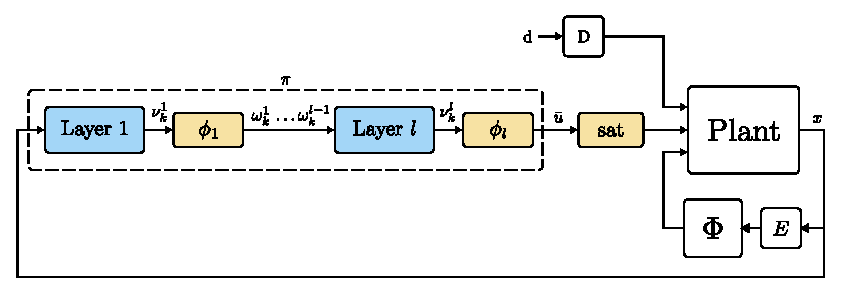
\includegraphics[width=0.65\textwidth]{img/first_scheme}
    \caption{Feedback system}
    \label{fig:first_scheme}
\end{figure}

The controller is implemented as a Multi Layer Perceptron with $l$ layers, each with $n_{\phi_i}$ neurons, all the activation functions are saturation functions, represented by $\phi_i$. The objective is to design an event-triggering mechanism that allows to ease the computational burden associated with the computation of many non-linear activation functions providing at the same time sufficient sector conditions to handle the non-linearity of the system and the controller. The controller $\pi$ is defined by:
\begin{equation}\label{eq:nn-equations}
  \begin{aligned}
  \omega^{0}(k) &= x(k) \\
  \nu^{i}(k) &= W^{i} \omega^{i - 1}(k) + b^{i}, i \in \left\{ 1, \dots, l \right\}\\
  \omega^{i}(k) &= \phi_i(\nu^i(k))\\
  \bar{u}(k) &= \phi_l(\nu^l(k))
  \end{aligned} 
\end{equation}
with $\nu^i(k) \in \RR^{n_{\phi_i}}$ the input to the $i$-th activation function $\phi_i: \RR^{n_{\phi_i}} \to \RR^{n_{\phi_i}}$, $\omega^i(k) \in \RR^{n_{\phi_i}}$ the output. The weights $W^i \in \RR^{n_{\phi_i} \times n_{\phi_{i-1}}}$ and biases $b^i \in \RR^{n_{\phi_i}}$ define the affine operation of each layer. The saturation function application is to be intended element-wise and will be denoted as $\phi_i(\nu^i(k)) = \left[ \varphi(\nu^i_1(k)), \dots, \varphi(\nu^i_{n_{\phi_i}}(k)) \right]$ and $\varphi: \RR \to \RR$ is the scalar activation function assumed to be symmetric and identical for every neuron. Adopting the same notation as in \cite{css-paper} we define the controller policy in a condensed form. Denoting the augmented vectors:
\begin{equation*}
  \nu_{\phi} = \bmx{\nu^1 \\ \vdots \\ \nu^l}, \omega_{\phi} = \bmx{\omega^1 \\ \vdots \\ \omega^l}, \phi_{\nu_{\phi}} = \bmx{\phi_1(\nu^1) \\ \vdots \\ \phi_l(\nu^l)} 
\end{equation*}
with $n_{\phi} = \sum_{i=1}^{l} n_{\phi_i}$ and $\phi: \RR^{n_{\phi}} \to \RR^{n_{\phi}}$ the combined non-linearity we have $\omega_\phi = \phi(\nu_\phi)$. Finally, conditions \ref{eq:nn-equations} can be rewritten as:
\begin{equation*}
  \bmx{u(k)\\ \nu_\phi(k)} = N \bmx{x(k) \\ \omega_\phi(k) \\ 1} 
\end{equation*}
where
\begin{equation}\label{eq:first-N}
  \bmx{
    \begin{array}{c | c c c c | c}
      \0 & \0 & \dots & \0 & W^l & b^l \\ 
      \hline
      W^1 & \0 & \dots & \0 & \0 & b^1 \\
      \0 & W^2 & \dots & \0 & \0 & b^2 \\
      \vdots & \vdots & \ddots & \vdots & \vdots & \vdots \\
      \0 & \0 & \dots & W^{l-1} & \0 & b^{l-1}
    \end{array}
  }
\end{equation}

Similarly as in \cite{css-extended} we implement an event-triggering-mechanism (ETM) in every layer of the controller, we add also a final ETM to the output that will be used to further reduce the total number of events and call to the non-linear functions. The system and the controller are now described by figure \ref{fig:second_scheme}.

\begin{figure}[H]
    \centering
    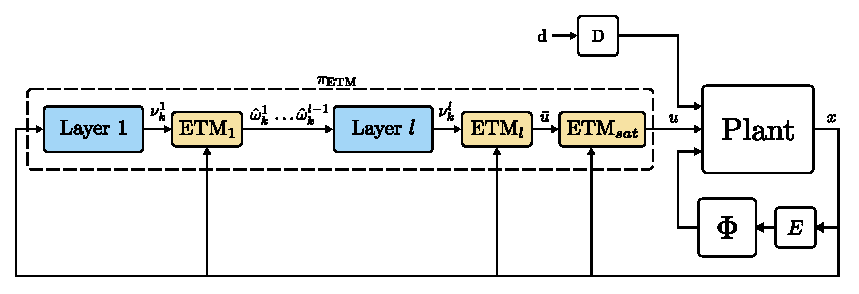
\includegraphics[width=0.45\textwidth]{img/second_scheme}
    \caption{Feedback system subject to ETM in the controller}
    \label{fig:second_scheme}
\end{figure}

The dynamics of the system are now described by:
\begin{equation}\label{eq:system-dynamics}
  x^{+} = A x + B u + C \Phi(E x) + D d
\end{equation}
with $u$ the output of the controller subject to the ETM. This modification required to redefine the matrix $N$ defined in the controller policy \ref{eq:first-N} as:
\begin{equation}\label{eq:last-N}
  N = \bmx{
    \begin{array}{c | c c c c | c}
      \0 & \0 & \dots & \0 & \Id & 0 \\ 
      \hline
      W^1 & \0 & \dots & \0 & \0 & b^1 \\
      \0 & W^2 & \dots & \0 & \0 & b^2 \\
      \vdots & \vdots & \ddots & \vdots & \vdots & \vdots \\
      \0 & \0 & \dots & W^l & \0 & b^l
    \end{array}
  } = \bmx{
    \begin{array}{c | c | c}
    N_{u x} & N_{u \omega} & N_{u b} \\
    \hline
    N_{\nu x} & N_{\nu \omega} & N_{\nu b}
    \end{array} 
  }
\end{equation}

The system is compliant with the assumptions of \textbf{Lemma 2} in \cite{css-extended} that allow us to define the following expressions regarding the equilibrium points $\left( x_*, u_*, \nu_*, \omega_* \right)$ of the system and controller given $x_*$, defining the matrices:

\begin{equation}
    \begin{aligned}
         R &= (\Id - N_{\nu \omega})^{-1}\\
         R_{\omega} &= N_{u x} + N_{u \omega} R N_{\nu x}\\
         R_b &= N_{u \omega} R N_{\nu b} + N_{u b}
    \end{aligned}
\end{equation}

With $N_{\nu \omega}$ always invertible due to its lower triangular structure. We express:

\begin{equation}
  \begin{aligned}
    u_* &= R_{\omega} x_* + R_b\\
    \nu_* &= R N_{\nu x} x_* + R N_{\nu b}\\
    \omega_* &= \nu_*
  \end{aligned}
\end{equation}

The equilibrium state $x^*$ needs some further discussion since the expression to retrieve it is no longer explicit due to the non-linearity $\Phi$. We can retrieve the vector using a numerical solver that minimizes the following expression for a given disturbance $\bar{d}$: 

\begin{equation}
  (A + B R_{\omega} - \Id) x_* + C \Phi(E x_*) + D \bar{d} + B R_b = 0
\end{equation}

\section{Main Results}

\subsection{Event-triggering mechanism}

\subsection{Lyapunov conditions}

\subsection{Optimization procedure}

\section{Simulations}

\section{Conclusions}

\printbibliography

\end{document}